\documentclass[11pt,a4paper,oneside,extrafontsizes]{memoir}

\renewcommand*{\baselinestretch}{1.04}
\isopage
\setlrmargins{*}{*}{1}
\checkandfixthelayout
%\documentclass[11pt,a4paper,twoside,openright,extrafontsizes]{memoir}

\renewcommand*{\baselinestretch}{1.04}
\isopage
\checkandfixthelayout
\usepackage{include/thesis}

\newcommand*{\bme}{Budapest University of Technology and Economics}
\newcommand*{\vik}{Faculty of Electrical Engineering and Informatics}

\newcommand*{\bmemit}{Department of Measurement and Information Systems}

\newcommand*{\vikdoctype}{Master's Thesis}
\newcommand*{\viktdkyear}{2017}

\newcommand*{\authors}{Author}
\newcommand*{\advisors}{Supervisors}

\newcommand*{\authori}{Dániel Stein}

\newcommand*{\advisori}{Gábor Szárnyas}
\newcommand*{\advisorii}{Ádám Lippai}

\title{Graph-Based Source Code Analysis of JavaScript Repositories}
\newcommand*{\titlepagetitle}{Graph-Based\\Source Code Analysis\\of JavaScript Repositories}
\author{\authori}

\hypersetup{
  pdftitle={\thetitle},
  pdfauthor={\theauthor, \advisors: \advisori, \advisorii}
  bookmarks=true,            % show bookmarks bar?
  unicode=true,              % non-Latin characters in Acrobat's bookmarks
  pdfnewwindow=true,         % links in new window
  colorlinks=true,           % false: boxed links; true: colored links
  linkcolor=black,           % color of internal links
  citecolor=black,           % color of links to bibliography
  filecolor=black,           % color of file links
  urlcolor=black             % color of external links
}


%\usepackage{marginnote}
%\usepackage{epigraph}
\usepackage[shortlabels]{enumitem}
\usepackage{placeins}
\usepackage{adjustbox}
\usepackage{booktabs}
\newcommand{\code}[1]{{\upshape\ttfamily\small\indent #1}}

\graphicspath{ {./include/figures/}, {./include/sources/} }

\usetikzlibrary{automata,arrows,positioning,trees,shapes.geometric}
\tikzset{
	>=stealth',
	stdstage/.style={
		rectangle,
		rounded corners,
		draw=black,
		minimum height=2.5em,
		text centered},
	processor/.style={
		diamond,
		minimum width=2em,
		minimum height=2em,
		aspect = 1,
		draw = black
		},
	flowedge/.style = {
		->,
		>=stealth',
		shorten >=1pt
	},
	textedge/.style={
		draw=none,
		text width = 7.5cm,
    inner sep = 1cm,
		align = left
	}
}

\bibliography{bibliography}

\begin{document}

\frontmatter{}

\thispagestyle{empty}

\begin{tikzpicture}[overlay,remember picture]
  \node at (current page.center) [yshift=1cm] {%
    \begin{minipage}{\textwidth}

      \centering

      \includegraphics[width=7cm]{include/figures/bme_logo}
      \vspace{0.3cm}

      \bme \\
      \vik \\
      \bmemit \\
      \vspace{3.5cm}

      {\Huge\sffamily\bfseries \titlepagetitle \par}
      \vspace{1cm}

      {\large \vikdoctype \par}
      \vspace{2cm}

      {\Large
        \authors: \\ \vspace{0.3cm}
        \authori

        \vspace{1cm}
        \advisors: \\ \vspace{0.3cm}
        \advisori \\
        \advisorii \\
        \advisoriii\par}

      \vspace{1.5cm}
      {\large \viktdkyear\par}

    \end{minipage}};
\end{tikzpicture}

\cleardoublepage

\tableofcontents

\selectenglish{}
\include{include/declaration}
\begin{otherlanguage}{magyar}

  \paragraph*{Kivonat}
  \phantomsection
  \addcontentsline{toc}{chapter}{Kivonat}
  \thispagestyle{plain}
  {
  \selecthungarian

  Egyre több, egyre inkább komplex szoftver vesz körül minket, amelyek gyakran kritikus rendszereket vezérelnek. Az ilyen rendszerek fő jellemzője, hogy a legapróbb hibáik is komoly következményekkel járhatnak. A forráskód statikus analízise egy, a kritikus szoftverrendszereknél általánosan elfogadott megközelítés, amely a hibák mihamarabbi megtalálását célozza meg. A statikus analízis már a fejlesztési folyamat korai szakaszaiban is alkalmazható, mivel nincs szükség a kód fordítására és futtatására az ellenőrzés véghezviteléhez. A megközelítést számos eszköz megvalósítja, amelyek képesek visszajelzést adni a potenciális hibahelyeken túl arról is, hogy a forráskód megfelel-e a kódolási szabályoknak és követelményeknek.

  Habár több statikus analízis eszköz is elérhető általános célú nyelvek elemzéséhez, és ezek gyakran a folytonos integráció részét képzik, JavaScript esetén ez nem mondható el annak dinamikus jellege miatt. A dinamikusan tipizált nyelvek sajátosságai miatt csak pár eszköz érhető el JavaScript forráskódok kódtárszintű statikus analíziséhez, illetve az eddig ismert ilyen eszközök nem nyújtanak egyszerre megoldást alaki és globális ellenőrzésre, futási utak meghatározására és folytonos integrációval történő alkalmazásra.

  Jelen dolgozatomban egy olyan, a folytonos integráció kiegészítésére képes keretrendszert tervezek, valósítok meg és értékelek, amely képes nagyméretű és gyakran változó Java\-Script forráskódtárak konfigurálható statikus analízisére. A keretrendszer alapjául szolgáló újszerű megközelítésnek köszönhetően az eddig megszokott megoldások helyett a felhasználók egyszerűbb módon fejezhetik ki az ellenőrzésre szánt követelményeket és képesek a több forráskódon átívelő követelményeket hatékonyabban ellenőrizni.

  }

\end{otherlanguage}

\cleardoublepage

\paragraph*{Abstract}
\phantomsection
\addcontentsline{toc}{chapter}{Abstract}
\thispagestyle{plain}

We are surrounded by more and more complex software that operate in mission-critical systems. Even small errors in these software can lead to serious consequences that may be too expensive to let happen. Static analysis is a proven approach for detecting mistakes in the source code early in the development cycle. Since static analysis does not compile or run the code, it can be applied at an early state of development. With static analysis it is possible to check whether the software conforms to the coding rules and requirements, and to locate potential errors.

While multiple static analysis tools exist for general purpose programming languages and these are generally part of the continuous integration systems, this is not the case with JavaScript. Due to the dynamically typed nature of this language there are only a few tools available for JavaScript codebases. Also, there are currently no tools available jointly providing lower level and global static analysis, finding control flows, and providing integration points for continuous integration systems.

In this report I design, implement and evaluate a framework extending the continuous integration workflow of large and frequently changing JavaScript repositories with configurable static analysis tools and techniques. Due to the novel approach of the framework, its users can express requirements easier and they are able to check global level requirements more efficiently.

\clearpage

\newcounter{savepage}
\setcounter{savepage}{\arabic{page}}

\mainmatter{}

\chapter{Introduction}
\label{chap:introduction}

\section{Context}
\section{Problem Statement and Requirements}
\section{Objectives and Contributions}
\section{Structure of the Thesis}

% !TEX root = ../main.tex
\chapter{Preliminaries}
\label{chap:preliminaries}

In this chapter I introduce the conceptual foundations and related technologies of my work. Here I discuss the building blocks required to create a static analyzer framework for JavaScript.

\section{JavaScript}
\subsection{ECMAScript 2015}
\subsection{WebAssembly}


\section{Static Analysis}
Even in 1995, the idea of static analysis was over 25 years old: \textquote[\cite{wichmann_industrial_1995}]{The idea  that  computer  software  should be used to analyse source programs rather than compile them, has a history of at least 25 years.}

Source code analysis can be used to discover facts about a particular program. Two basic automated analysis methods exist for source code analysis:
\begin{itemize}[topsep=0pt]
  \item \emph{Static analysis} is performed by reading the source code and analyzing it without evaluating the statements or executing the program.
  \item \emph{Dynamic analysis} is performed by executing the program and evaluating its output for given input sequences.
\end{itemize}

% > The term is usually applied to the analysis performed by an automated tool, with human analysis being called program understanding, program comprehension, or code review. Software inspections and Software walkthroughs are also used in the latter case.
% https://en.wikipedia.org/wiki/Static_program_analysis

While JavaScript is usually not compiled, high-level language source codes are audited at least by the compiler. Thus a specific static analysis should aim to discover unwanted traits of the source in ways a generic compiler could not do, resulting in better code quality. These treats, \emph{bugs} are usually perceptable while running the code. Another way to locate these bugs is to write and run tests, dynamically testing the program.
% \cite[][72]{wichmann_industrial_1995}

The two analysis methods are complementing each other. They discover different subsets of problematic constructions. Information discovered during the static analysis may be used later in the dynamic testing.

% > Static analysis bug-finding tools have evolved over the last several decades from basic syntactic checkers to those that find deep bugs by reasoning about the semantics of code. The goal of the Clang Static Analyzer is to provide a industrial-quality static analysis framework for analyzing C, C++, and Objective-C programs that is freely available, extensible, and has a high quality of implementation.
% http://clang-analyzer.llvm.org/


\subsection{Use Cases}
Static analysis tools employ diverse levels of abstraction. \emph{Formatters} make sure that the source code complies with the style guide. \emph{Linters} check for stylistic and programming errors and warn at suspicious programming constructs. \emph{Formal verification}, on the other hand, utilizes formal mathematical methods to prove or refute statements about the source code and its behavior.

For dynamic languages, it can be used for even more: finding previously undefined property reads, catching invokement of non-functional variables~\cite{jensen_type_2009}, detecting dead code, and so on.

\subsection{Advantages and Disadvantages}

Since static analysis tools deliberately do not evaluate the source code, there are fundamental limitations to what problems they can discover. I consider the following advantages and disadvantages important.


\subsubsection{Advantages}
\paragraph{Input Data Is a By-Product of Compilers}

\paragraph{No Need for Execution}
\begin{itemize}
  \item no need for run environment
  \item no need for mocking, emulating
\end{itemize}

\subsubsection{Disadvantages}
\paragraph{Speed} Static analysis trades CPU time and memory for better code quality. By design it may be multiple orders of magnitude slower than compilation, but its speed depends not only on the underlying data structure and algorithms, but also the level of analysis.
%  > Slower than Compilation
%
%  > Operationally, using static analysis to automatically find deep program bugs is about trading CPU time for the hardening of code. Because of the deep analysis performed by state-of-the-art static analysis tools, static analysis can be much slower than compilation.
%
%  > While the Clang Static Analyzer is being designed to be as fast and light-weight as possible, please do not expect it to be as fast as compiling a program (even with optimizations enabled). Some of the algorithms needed to find bugs require in the worst case exponential time.

However, with a given limitation of granularity, in case of a source code modification, previous results can be reused. There is a possibility that only the modified---and other affected---parts need to be processed again. The incremental approach of static analysis may speed up the process by orders of magnitude~\cite{stein-daniel-bsc}.

\paragraph{False Positives} Static analysis can not prove the correctness of a source code. It rather warn in case there is a possibility of a problem. Thus static analysis tools can introduce false positive warnings and flag code parts as problematic even if they behave correcly.

To reduce the number of false positive warnings, one usually introduces more precise, specified rules and more thorough analysis.

%  > False Positives
%
%  > Static analysis is not perfect. It can falsely flag bugs in a program where the code behaves correctly. Because some code checks require more analysis precision than others, the frequency of false positives can vary widely between different checks. Our long-term goal is to have the analyzer have a low false positive rate for most code on all checks.
%
%  % http://clang-analyzer.llvm.org/

\subsection{Source Code Processing and Analysis}
\label{sect:source-code-processing}
The source code of a program is a sequence of instructions formulated in a programming language as a text. Grammars of formal languages are a set of rules describing what the compiler considers a valid input---how to create valid instructions or a set of instructions from the alphabet of the language \emph{(syntax)}. A source code processing entity (transformer, or hereafter \emph{compiler}) assigns a meaning \emph{(semantics)} and transforms the instruction to another language (generally an intermediate language or bytecode).

What input data the compiler considers useful information depends on the semantics of the language the compiler is built for. Source codes contain a much wider variety of data than a compiler requires for transforming, analyzing the application: comments, function declaration order, indentation, line breaks all help the reader (and writer) of the code, but carry no additional information.

\Cref{fig:processing-the-source-code} shows the general process for processing source code and transforming a stream of characters into a data structure with \emph{meaning}.

\begin{figure}[!ht]
	\centering
	\adjustbox{max width=\textwidth} {
		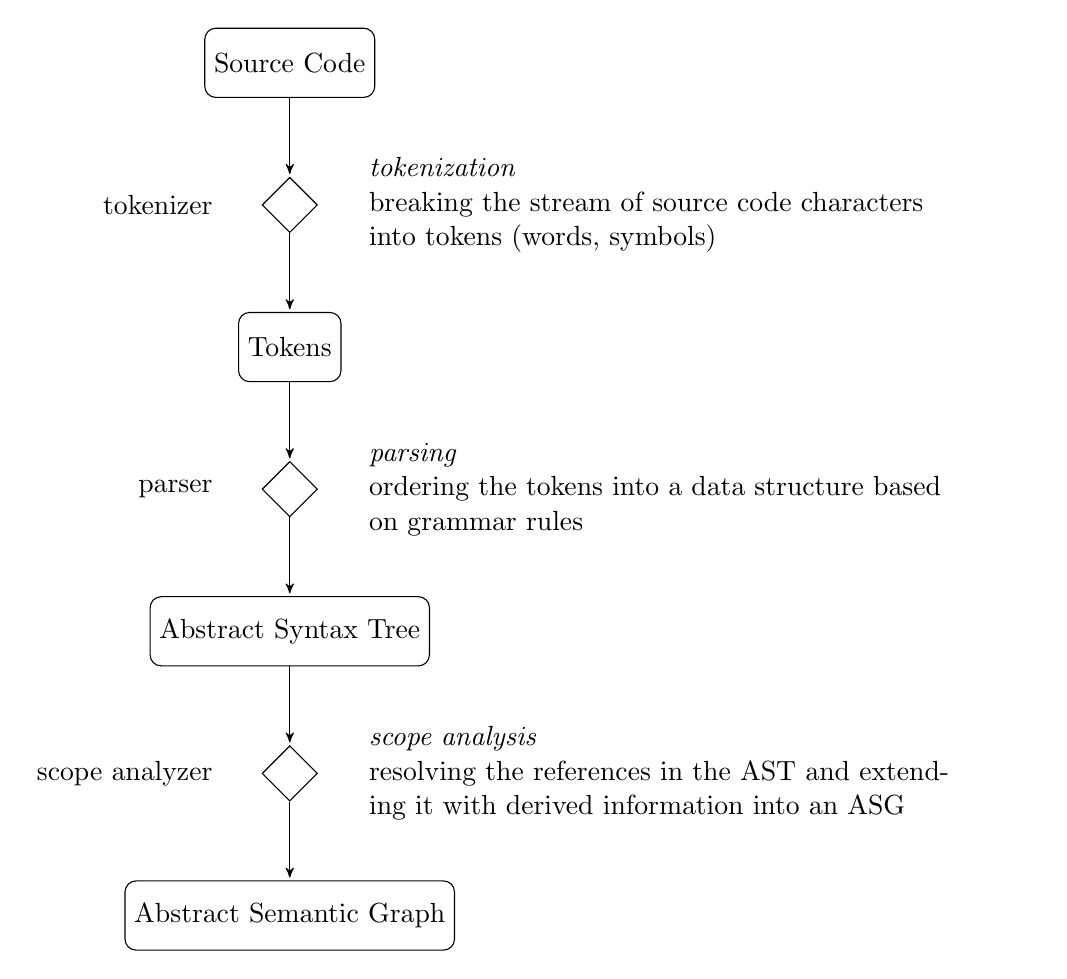
\begin{tikzpicture}[
			node distance = 1cm,
      label distance = 0.5cm,
			auto,
			]

    \node[stdstage] (SC) {Source Code};
    \node[processor,
          below=of SC,
          label={left:tokenizer}
          ] (TOK) {};
    \node[stdstage, below=of TOK] (TO) {Tokens};
    \node[processor,
          below=of TO,
          label={left:parser}
          ] (PAR) {};
    \node[stdstage, below=of PAR] (AST) {Abstract Syntax Tree};
    \node[processor,
          below=of AST,
          label={left:scope analyzer}
          ] (SA) {};
    \node[stdstage, below=of SA] (ASG) {Abstract Semantic Graph};


    \path (SC) edge[flowedge]  (TOK);
    \path (TOK) edge[flowedge] (TO);
    \path (SC) edge[textedge] node {\emph{tokenization}\\ breaking the stream of source code characters into tokens (words, symbols)} (TO);

    \path (TO) edge[flowedge]  (PAR);
    \path (PAR) edge[flowedge] (AST);
    \path (TO) edge[textedge] node {\emph{parsing}\\ ordering the tokens into a data structure based on grammar rules} (AST);

    \path (AST) edge[flowedge]  (SA);
    \path (SA) edge[flowedge] (ASG);
    \path (AST) edge[textedge] node {\emph{scope analysis}\\ resolving the references in the AST and extending it with derived information into an ASG} (ASG);
		\end{tikzpicture}
	}
	\caption{Processing the source code}
	\label{fig:processing-the-source-code}
\end{figure}

\subsubsection{Lexical Analysis}
A \emph{lexer}, \emph{tokenizer}, or \emph{scanner} forms the first phase of a parsing process. It scans the input character stream and segments them into sequence of groups, tokens, \emph{strings with a ``meaning''}. It also categorizes these groups into various token classes, token types. Processing the raw input into a value (converting the string \code{"2"} into the number $2$) can also happen in this phase. \Cref{fig:tokenization} shows how an expression string can be tokenized.

\begin{figure}[!htb]
  \centering
  \code{foo = 1 / 0}\\[1em]

  \begin{tabular}{c|l}
    Token & Token type\\
    \hline
    \code{foo} & \code{IDENTIFIER (Ident)}\\
    \code{=} & \code{ASSIGN (Punctuator)}\\
    \code{1} & \code{NUMBER (NumericLiteral)}\\
    \code{/} & \code{DIV (Punctuator)}\\
    \code{0} & \code{NUMBER (NumericLiteral)}\\
    \hline
  \end{tabular}

  \caption{Character stream and tokenization result with token type information}
  \label{fig:tokenization}
\end{figure}


\subsubsection{Parser}
A \emph{parser} forms the second phase of a parsing process, using the output token stream of the \emph{lexer}. It takes the input data and builds a hierarchical data structure (a \emph{parse tree} or an \emph{abstract syntax tree}) representing the input. If the input does not comply with the syntax rules, thus an tree can not be built, the source code is syntactically incorrect.

\Cref{fig:sentence-s-expression} shows a sentence and its s-expression representation. S-expressions (for ``symbolic expression'') are a notation for tree-structured nested list, mainly used in Lisp.

\begin{figure}[!htb]
\centering
\code{The quick brown fox jumps over the lazy dog}\\[1em]

\begin{minipage}{3cm}
\begin{verbatim}
(Sentence
  (Word The)
  (Word quick)
  (Word fox)
  (Word jumps)
  (Word over)
  (Word the)
  (Word lazy)
  (Word dog)
)
\end{verbatim}
\end{minipage}
  \caption{A sentence and its s-expression representation}
  \label{fig:sentence-s-expression}
\end{figure}

\paragraph{Abstract Syntax Tree}
An \emph{Abstract Syntax Tree} (AST) is a tree representation of the syntactic structure of the result of a parsing along a grammar. The nodes of the tree denote a construct occuring in the input, while the edges represent the connection between these nodes based on the grammar rules.

As mentioned in~\cref{sect:source-code-processing}, source code contains much more detail (e.g., indentation, whitespace, comments) than is required and restrained during the parsing process. Thus this representation is a digested, \emph{abstract} syntax tree. It may be transformed based on transformation rules and source code can be generated from ASTs. Without restraining the layout information and reusing it during the code generation, the resulting text can show differences in indents, whitespaces and expression formulation compared to the initial source code.

\Cref{fig:ast-asg-example} shows an example AST (in black), where a one-statement JavaScript file is parsed. The content of the file was only \code{var foo = 1 / 0;}.

\subsubsection{Scope Analyzer}
A \emph{scope analyzer} or \emph{context analyzer} produces a data structure that represents the scoping information of a program, probably extending the information available from an AST or an ASG. An element representing a scope in this data structure may contain, inter alia, metadata about the scope itself, the AST node related to the scope, available assets (variables, functions, etc.) in that scope.~\cite{shift-scope}

\paragraph{Abstract Semantic Graph}
As its name implies, an \emph{Abstract Semantic Graph} (ASG), although sounding alike, differs from an Abstract Syntax Tree. (1) ASGs are graphs, and (2) express more than the syntactic information; ASGs carry semantic information expressed with additional edges. These edges can not exist in an AST, as they are non-tree edges (cross-edges). For example they may connect variable references to their declarations.~\cite{raghavan_dex:_2004}

An ASG is a graph representation of a parse result; the nodes represent subterms of an expression. Shared subterms can occur, having more than one node linked to the same, common subterm. Compilers generally work on ASGs internally, since not only the syntactical, but the behavioral information are also represented in them.

% An abstract semantic graph is typically constructed from an abstract syntax tree by a process of enrichment and abstraction. The enrichment can for example be the addition of back-pointers, edges from an identifier node (where a variable is being used) to a node representing the declaration of that variable. The abstraction can entail the removal of details which are relevant only in parsing, not for semantics.
% https://en.wikipedia.org/wiki/Abstract_semantic_graph

\Cref{fig:ast-asg-example} shows the difference between an AST and an ASG (in turquoise).

\begin{figure}[!htb]
	\centering
	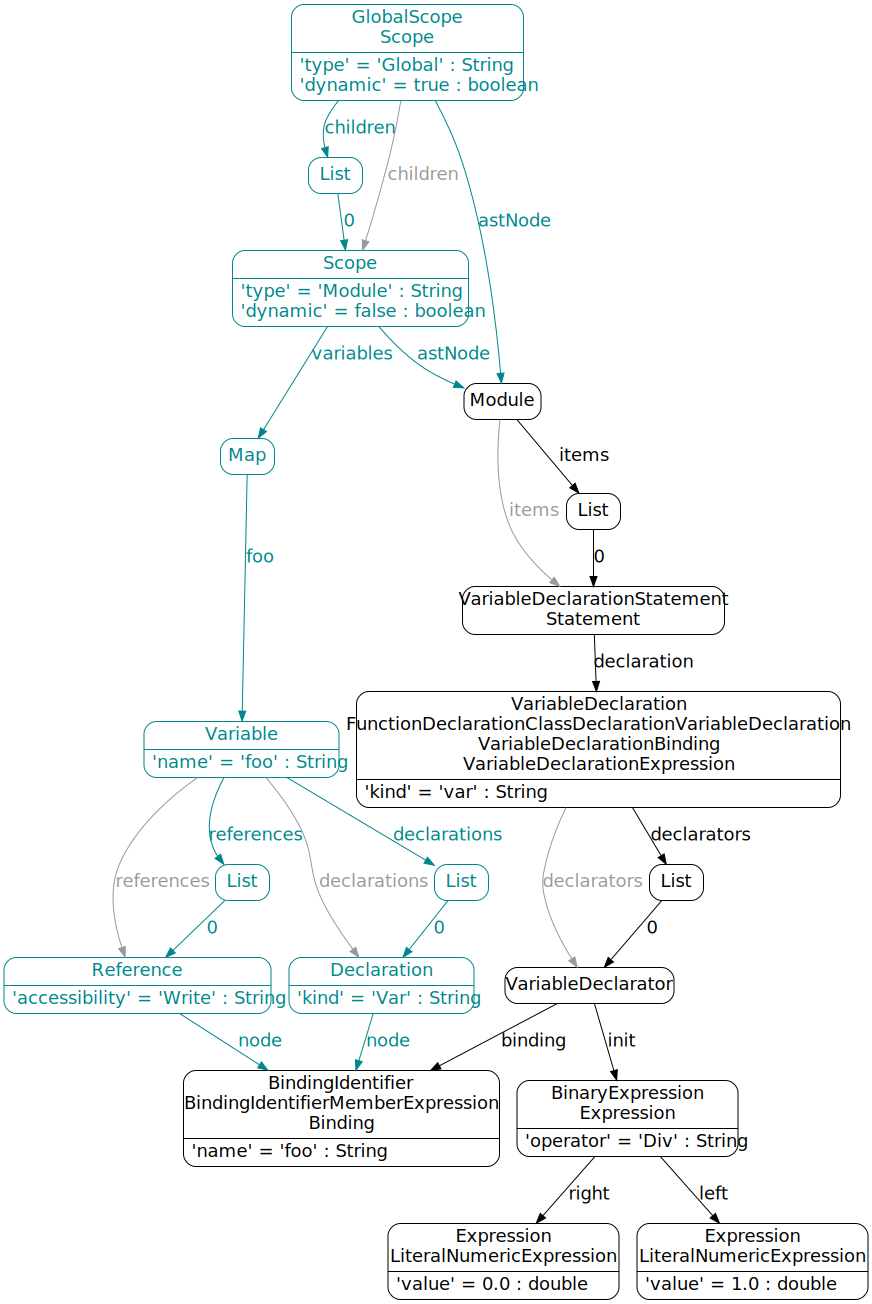
\includegraphics[height=\textheight, trim=1cm 1cm 1cm 1cm,clip]{include/figures/AST-ASG}
	\caption{AST (in black) with additional edges (ASG, in turquoise) and derived helper edges (in gray).}
	\label{fig:ast-asg-example}
\end{figure}

\FloatBarrier

\section{Type Inference}

Type inference refers to the deduction of the data types of expressions, statements during static analysis.

> Type inference refers to the automatic deduction of the data type of an expression in a programming language. If some, but not all, type annotations are already present it is referred to as type reconstruction[citation needed]. The reverse operation of type inference is called type erasure.

> It is a feature present in some strongly statically typed languages. It is often characteristic of functional programming languages in general. Some languages that include type inference are Nim, ML, OCaml, F\#, Haskell, Scala, Go, D, Clean, Opa, Rust, Swift, Visual Basic (starting with version 9.0), C\# (starting with version 3.0) and C++11. The ability to infer types automatically makes many programming tasks easier, leaving the programmer free to omit type annotations while still permitting type checking.

% https://en.wikipedia.org/wiki/Type_inference

\subsection{Typed JavaScript Derivations}

\subsection{Analysis of JavaScript Source Codes}
There are several static analysis frameworks and solutions available for JavaScript. I introduce and compare them in detail in \cref{sect:javascript-parsers} (JavaScript parsers) and \cref{sect:javascript-type-inferencers} (JavaScript type inferencing solutions).


\section{Handling Large Interconnected Data}
The progress of computer parts -- the ever increasing amount of processing power, and memory and storage speed and sizes -- and the alike growth of data to be stored and processed during the last more than fifty years yielded various solutions.

Based on historic evolution, these solutions can be categorized in three main categories:
\begin{itemize}[topsep=0pt]
  \item \emph{Navigational} database management systems (DBMS) were mainly used in the era of magnetic tape based storages, in which the \emph{records} contained references to other records allowing the system to fast-forward, \emph{navigate} there and load additional data.

  \item \emph{Relational} DBMSs organizes data in a \emph{relational model}~\cite{codd}, where one or more \emph{relations} contain unique entries (\emph{records} or \emph{tuples}).

  Relational databases leverage precise mathematical background (see \emph{relational algebra} and \emph{relational calculus}), have diverse implementations, mature tooling, and data access security by authentication and authorization. There are also disadvantages; due to their data structure, relational databases may have scalability and performance issues. They are also typically optimized for transactional processing and not data analysis (there are exceptions, see \emph{data warehouses}).

  \item \emph{Post-relational} databases is a vague collective name for every database system that abandons the strictness and burden of the relational data model and the Structured Query Language (SQL).

  Since the turn of the millennium, the struggle with storing and processing huge amounts of data using relational technologies spawned a diverse palette of new database management systems using simpler, more scalable data models. These systems are consequently called \emph{non SQL}, NoSQL databases, and are increasingly used in real-time and big data applications.

  NoSQL systems are a heterogeneous set of systems, with very different approaches. Categories of these systems based on their data models include, but are not limited to: \emph{key-value stores}, \emph{wide column stores}, \emph{document stores}, \emph{graph DBMSs}, \emph{RDF stores}.
\end{itemize}

Since my approach is based on graph databases, in this section I introduce the concept of graph databases, and graph pattern matching. I also introduce several graph database implementations and systematically compare them in order to select the appropriate technology for the approach.


\subsection{On Graph Computing}
Graphs are well-known and in computer science widely used mathematical concept, which has been around for many decades. Numerous graph technologies have evolved, each with their advantages and disadvantages. From graphs themselves to physical and virtual worlds, many scenarios can be represented as graphs and stored in graph databases with their respective data model. This section loosely follows~\cite{scm, On_Graph_Computing}.

\begin{figure}[!ht]
	\centering
	\includegraphics[width=0.8\textwidth]{include/figures/graph-classes}
	\caption{Graph data models~(based on~\cite{DBLP:journals/corr/abs-1006-2361}).}
	\label{fig:graph-classes}
\end{figure}

The most basic graph model is the \emph{simple graph}, formally defined as $G = (V, E)$, where $V$ is the set of vertices and $E \subseteq V \times V$ is the set of edges. Simple graphs are sometimes referred as textbook-style graphs because they are an integral part of academic literature. Simple graphs are useful for modeling homogeneous systems and have plenty of algorithms for processing.

Simple graphs can be extended in several different ways (see \cref{fig:graph-classes}). To describe the connections in more detail, one may add directionality to edges (\emph{directed graph}). To allow different connections, one may label the edges (\emph{labeled graph}).

\emph{Typed graphs} introduce types for vertices. \emph{Property graphs} (sometimes called \emph{attributed graphs}) add even more possibilities by introducing properties. Each graph element, both vertices and edges can be described with a collection of properties. The properties are key--value pairs, e.g.\ \texttt{type = `Person'}, \texttt{name = `John'}, \texttt{age = 34}. \emph{Semantic graphs} use Uniform Resource Identifiers (URIs) instead of labels, otherwise they have similar expressive power as labeled graphs.

My approach utilizes typed (labeled) property graphs.

\subsubsection{Graph Computing Technologies}
The practice of data storage and processing is encumbered with space and time trade-off. This trade-off is also present in various graph computing technologies. This section discusses the categorization of these technologies and mentions a few technologies of which the most popular ones are detailed in~\cref{sect:graph-databases}.

The landscape of graph storing and processing solutions is populated and diverse (see~\cite{zhang_-memory_2015}). The basic categorization of software graph database solutions is the following. Graph computing technologies can be divided into two groups: on-line, real-time; and global analyzing, batch-processing graph databases. The former can be divided into in-memory, and persistent databases.

\paragraph{In-Memory Graph Toolkits}
The challenge of big data problems shed light on that the existing disk-based systems can not offer timely response due to the latency of hard disks. The role of storage shifted from the hard drive to the memory of the system. In-memory graph databases are constrained to graphs that fit into the main memory. Thus these systems are single-user systems that are oriented towards low-latency graph analysis.

The locality of data allows the usage of rich algorithm libraries and the choice of the adequate graph representation with respective space-time trade-off. The constraint of space allows large graphs (with millions of edges) to be stored and processed, but this is not sufficient in all cases.

Example in-memory graph toolkits: \emph{Apache Giraph}, \emph{Microsoft Graph Engine} (formerly \emph{Trinity}), \emph{Apache Spark GraphX}, \emph{WhiteDB}.

\paragraph{Persistent, Real-Time Graph Databases}
Persistent graph databases are the prevalent group of graph computing technologies. Unlike in-memory graph tools, graph databases persist data on the hard drives, thus they can support billions of edges on a single machine and distributed systems can handle hundreds of billions of edges. These databases can provide multi-user concurrency, transactional semantics and eventual consistency.

Since global graph algorithms are not feasible, these systems are optimized for local neighborhood analysis and concurrent access. Global graph analytics are inefficient due to the communication overhead and the computational overhead, e.g., transactional semantics.

Example for persistend, real-time graph databases: \emph{InfiniteGraph}, \emph{Neo4j} (see \cref{sect:neo4j}), \emph{OrientDB} (see \cref{sect:orientdb}), and \emph{Titan} (see \cref{sect:titan}).

\paragraph{Batch-Processing Graph Frameworks}
In case there is no real-time requirement for the analysis touching the whole dataset, batch-processing graph frameworks can be used for global analytics. Since there is no burden of being real-time, the applied algorithm can even scan data multiple times and leverage sequential reads from the disk. These systems can be used to periodically process data and feed back the results into real-time graph databases. Most of these frameworks utilize Hadoop for storage (HDFS) and processing (MapReduce).

Example batch-processing graph frameworks: \emph{Apache Hama}, \emph{Apache Giraph}, and \emph{DataStax Aurelius Faunus}.


\subsection{Evaluating Queries on a Data Structure}
Numerous strategies exist for defining and executing queries over data structures. They can be defined in an imperative manner with programming languages like a navigation described in \emph{Gremlin} over a graph database or using a data access interface such as the Eclipse Modeling Framework. Declarative solutions also exist, where the query plan is calculated from the query formalized in a declarative language (like \emph{SQL}, \emph{SPARQL}, \emph{Cypher}) and execution is performed by a query framework (such as \emph{4store}, \emph{Neo4j}). Graph pattern matching -- one of the declarative querying solutions, supplemented by imperative logic -- forms the foundation of my approach.

\subsubsection{Graph Pattern Matching}
\textquote[\cite{csmr}]{Graph patterns are a declarative, graph-like formalism representing a condition (or constraint) to be matched against instance model graphs. The formalism is useful for various purposes in model-driven development, such as defining model transformation rules or defining general purpose model queries including model validation constraints. A graph pattern consists of structural constraints prescribing the interconnection between nodes and edges of a given type.

A match of a pattern is a tuple of pattern parameters that fulfill all the following conditions:
\begin{enumerate}[topsep=0pt]
	\item have the same structure as the pattern,
	\item satisfy all structural and attribute constraints,
	\item and does not satisfy any negative application condition (NAC) describing cases when the original pattern does not hold.
\end{enumerate}}


\subsection{Graph Databases}
\label{sect:graph-databases}
Since my thesis work is based on graph-based data handling, it is essential to use a technique that is suitable. In this case suitable is better described as being fast, flexible, versatile, easy to use and deploy. In this section I go over some of the most promising candidates and justify why I have chosen Neo4j as the foundation of my approach.

\subsubsection{Neo4j}
\label{sect:neo4j}
Neo4j is one of the most popular and most mature NoSQL graph databases developed by \emph{Neo Technology}. It is open-source, well-documented and steadily-developed. Neo4j is available in two editions: a free \emph{Community Edition} and a paid \emph{Enterprise Edition}.~\cite{neo4j}

\paragraph{Architecture}
Since Neo4j was written in Java (and Scala), it can be used to start a new project quick and easy. In respect of connection, it can be deployed two ways: in \emph{server mode} the database is started separately and listens for queries on its HTTP REST and Bolt interface; where in \emph{embedded mode} it runs in the same JVM as the only client application.

\paragraph{Data Model}
The graph model in Neo4j, \code{Neo4jGraph} is an implementation of the \emph{TinkerPop} graph computing framework's \emph{Blueprints} property graph data model. More precisely it is a labeled property graph, since the relations are labeled and the nodes can also hold multiple labels; the nodes and relations can both hold properties.

Unfortunately the relations are only binary, ternary (and n-ary $n>2$) relations can only be stored with an introduced indirection, a connection node connecting every node in the relation.

\paragraph{Sharding}
Although the \emph{Enterprise Edition} of Neo4j has a high availability solution and supports clustered replication and cache sharding, it does not support sharded data storage over a cluster of devices. This results in the advantage of low latency (clustering provides scale out capabilities for read), the ability to handle transactions and having ACID as the consistency model.~\cite{neo4j-product}

\paragraph{Query Language}
Neo4j provides two methods for data query out-of-the-box: an object-oriented native Java API for graph navigation and Cypher, a graph pattern description and query language with declarative and imperative traits. Additional interfaces may be loaded as a plugin, like the imperative Gremlin query interface~\cite{neo4j-gremlin-plugin}.

One of Cypher's best features is the readibility of its syntax. It provides an intuitive way to describe patterns of nodes and relations in the graph and also connections between subpatterns using bound identifiers for nodes and relations. Cypher also manages the indexes and constraints of the graph database. Negative application conditions (NAC) can be also expressed, describing the cases where the query should not return a match.

Other interesting and useful features of Cypher includes:
\begin{itemize}[topsep=0pt]
  \item Repetition bound (or unbound) transitive closure over an edge. The label of the edge can be also set to one label or a set of labels. Given sequence of labeled edges (with or without bound labels of nodes) can not be set on its own, but temporary edges can be utilized to emulate this behavior.
  \item Stored procedures are a very welcome new feature of the latest (as of May, 2016) Cypher and Neo4j version (v3.0). Procedures written in Java can be stored in the server as a plugin and called from the queries abolishing the need for manual logic-based calls in case it was not possible to formalize a query for it (ranging from duplicating a node (with parameters and labels) to infering the metamodel (from the nodes and relations already in the database)).
  \item Parametrized queries may be utilized for faster evaluation.
  \item List predicates evaluating predicates for all/any/none or single one nodes of the path.
  \item Iterating and unwinding a collection in the query
  \item Finding the shortest path
  \item Mathematical functions
  \item Query profiling
\end{itemize}

\textquote[\cite{neo4j-developer}]{Since October 2015 the openCypher project aims to provide an open grammar, language specification, technical compatibility kit and reference implementation of parser, planner and runtime for Cypher.}

\paragraph{Other Advantages and Disadvantages}
\begin{itemize}[topsep=0pt]
  \item[+] When Neo4j is deployed in server mode, besides the REST and Bolt interfaces, a web GUI is also available, where a read-evaluate-print loop (REPL) interface helps the user with interactive querying. The results are either shown in a table or an also interactive graph display, where the user can automatically add necessary nodes and relations from the database (without explicitly executing another query). It also supplies the user with information about the contents of the database, labels, indexes.
  \item[+] Graph Gists are interactive teaching tools allowing the visitor of the site to learn about various domains modeled in Neo4j and learn from the example queries.
\end{itemize}

\subsubsection{Titan}
\label{sect:titan}
\textquote[\cite{titan}]{Titan is a scalable graph database optimized for storing and querying graphs containing hundreds of billions of vertices and edges distributed across a multi-machine cluster. Titan is a transactional database that can support thousands of concurrent users executing complex graph traversals in real time.}

Titan was developed by \emph{Aurelius} until the company was aquired by \emph{DataStax} in 2015. DataStax has expressed its intentions to preserve the effort made by front-end users dependent on Titan and ensures the current users that the foreseeable merging procedure to DataStax Enterprise solutions will be as simple as possible~\cite{titan-datastax-acquirement}.

\paragraph{Architecture}
\textquote[\cite{titan-arch,titan-benefits}]{Titan is designed to support the processing of graphs so large that they require storage and computational capacities beyond what a single machine can provide. Titan implements robust, modular interfaces for data persistence, data indexing, and client access. Titan’s modular architecture allows it to interoperate with a wide range of storage, index, and client technologies; it also eases the process of extending Titan to support new ones.}

Titan is based on one or more disk-based storage and indexing adapters. Titan comes out-of-the-box with 3 data storage adapters: \emph{Cassandra}, \emph{HBase}, and \emph{BerkeleyDB}; and also 2 indexing adapters: \emph{Elasticsearch} and \emph{Lucene}. These indexing adapters speed up and enable more complex queries.

Like Neo4j, applications based on Titan can also interact with it in two ways~\cite{titan-arch}:
\begin{itemize}[topsep=0pt]
  \item Embedding Titan in the application allows direct querying against the graph within the same JVM. In this case query execution, caching, transaction handling all happens in the same JVM. The data retrieval from the storage adapters can be either local or remote.
  \item With a local or remote Titan instance one can interact by submitting Gremlin queries to the server.
\end{itemize}


\paragraph{Data Model}
Titan natively supports the property graph data model exposed by \emph{TinkerPop}.

\paragraph{Sharding}
Since Titan can be used with Cassandra as the data storage adapter, the architecture inherits every one of Cassandra's advantages. It is possible to set up a highly available Titan cluster with no single points of failure. This configuration also utilizes the Cassandra's partitioner (a hash-based, sophisticated partitioning system).

Using multiple storage backend servers eliminates read (and sometimes write) bottlenecks as these servers can serve data for the same query in a coordinated manner utilizing that the architecture lacks the master/slave layout. A caching layer ensures the availability of the most used data parts from the memory cache speeding up the queries even more. Elastic scalability allows the introduction and removal of machines to the live cluster.


\paragraph{Query Language}
Titan natively supports the imperative graph traversal language Gremlin (by \emph{TinkerPop}).


\subsubsection{OrientDB}
\label{sect:orientdb}
\paragraph{Architecture}
\paragraph{Data Model}
\paragraph{Sharding}
\paragraph{Query Language}


\subsubsection{4store}
\paragraph{Architecture}
\paragraph{Data Model}
\paragraph{Sharding}
\paragraph{Query Language}


\subsubsection{Stardog}
\paragraph{Architecture}
\paragraph{Data Model}
\paragraph{Sharding}
\paragraph{Query Language}

\subsection{A Viable Alternative: EMF Modeling and VIATRA Query}
Although EMF is not a graph database, with the help of VIATRA Query, the data stored in an EMF instance model can be queried like graph databases.

\subsubsection{Modeling}
Modeling is a versatile concept, the word itself may refer to various topics. In the context of this thesis, by models I primarily mean data models. A data model---or sometimes called domain model---organizes the data elements, how they relate to each other and what actions one can perform on them.

\paragraph{Metamodels and Instance Models}
\textquote[\cite{scm}]{Metamodeling is a methodology for the definition of modeling languages. A metamodel specifies the abstract syntax (structure) of a modeling language. Metamodels are expressed using a metamodeling language that itself is a modeling language. The metamodel can also be interpreted as the object-oriented data model of the language under design. Metamodeling can be viewed as the grammar for a \emph{typed property graph}, so the created models are both \emph{typed graph}s and \emph{property graph}s.}

The metamodel contains the main concepts and relations of the domain specific language (DSL) and defines the possible structure of the instance models. To enrich the expressive power of the language, attributes are added to the concepts. By doing this, the language can be extended with predefined domains of data types (like integers, strings) that are supported by the metamodeling language. Additionally, some structural constraints might be specified with the elements like multiplicity.

Models describing a particular problem in the domain, called instance models, are defined using the elements of the metamodel.

\subsubsection{The Eclipse Modeling Framework}
\label{sect:emf}
Eclipse is a free, open-source software development environment and a platform with extensible plug-in system for customization. Eclipse comes with its own modeling tools, with the core framework called Eclipse Modeling Framework (EMF).

\textquote[\cite{EMF}]{The EMF project is a modeling framework and code generation facility for building tools and other applications based on a structured data model. From a model specification described in XMI, EMF provides tools and runtime support to produce a set of Java classes for the model, along with a set of adapter classes that enable viewing and command-based editing of the model, and a basic editor. EMF (core) is a common standard for data models, many technologies and frameworks are based on.}

\paragraph{Ecore}
Ecore is the metamodeling language used by EMF. It has been developed in order to provide an approach for metamodel definition that supports the direct implementation of models using a programming language. Ecore is the de facto standard metamodeling environment of the industry, and several domain-specific languages are defined using this formalism.~\cite{scm}

\begin{figure}[!ht]
	\centering
	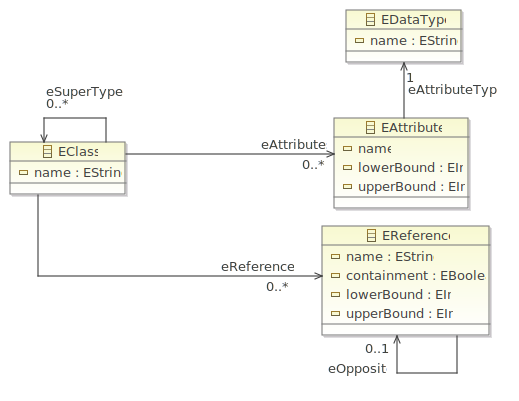
\includegraphics[height=10cm]{include/figures/Ecore}
	\caption{An illustrative core part of Ecore, the metamodeling language of EMF}
	\label{fig:Ecore}
\end{figure}

\Cref{fig:Ecore} shows only a small fraction of the metamodel, as there is many more classes in the Ecore metamodel. The main classes are the following:
\begin{itemize}[topsep=0pt]
	\item \code{EAttribute} represents a named attribute literal, which also has a type.
	\item \code{EClass} represents a class, with optional attributes and optional references. To support inheritance, a class can refer to a number of supertype classes.
	\item \code{EDataType} is used to represent simple data types that are treated as atomic (their internal structure is not modeled). Data types are identified by their name.
	\item \code{EReference} represents a unidirectional association between \code{EClass}es and is identified by a name. It is also possible to mark a reference as a containment that represents composition relation between elements. A bidirectional association should be modeled as two \code{EReference} instances mutually connected via their opposite references.
\end{itemize}

An Ecore model has a root object, representing the whole model. The children of this root object are packages, and the children of those are classes.

More detailed illustrations of the metamodel can be found in the EMF Documentation~\cite{ecore}.


\subsubsection{VIATRA Query}
VIATRA is an event-driven and reactive model transformation platform. \textquote[\cite{viatra}]{The VIATRA framework supports the development of model transformations with specific focus on event-driven, reactive transformations and offers a language to define transformations and a reactive transformation engine to execute certain transformations upon changes in the underlying model. Furthermore, the underlying incremental query engine, originating from the EMF-IncQuery project is reusable in different scenarios not related to model transformations.}

VIATRA Query (formerly IncQuery) is an incremental query engine with its own graph pattern based query language to specify and execute model queries on EMF instance models or other data storage solutions.

Since the data model of my approach may change over time, an unstructured or semi-structured data storage suits it better. EMF would require the metamodel to be transformed each time it is changed. It is also not possible to shard large EMF models in and take advantage of a clustered environment.


\section{Visual Studio Code}
Visual Studio Code~\cite{vscode} is Microsoft's take on a lightweight, yet powerful Integrated Developer Environment (IDE) for modern programming languages. It is available for free for Windows, OS X and Linux. It comes with built-in support for JavaScript, TypeScript and has a growing ecosystem of extensions for other languages, theming, and developer support~\cite{vscode-extensions}.

Debugging is also made easy, as the editor can be attached to the running code and the developer can add break points, look at call stacks and evaluate statements with an interactive console. With the relatively small package, Git support comes built-in: reviewing changed lines, staging files, making commits can be made right in the IDE.

\subsection{IntelliSense}
Visual Studio Code's syntax highlighting and autocomplete system is called IntelliSense, that also provides better completition based on variable types, function definitions, and imported modules. IntelliSense provides syntactical features like \emph{format on type}, \emph{outlining}; and also language service features like \emph{peek}, \emph{go to definition}, \emph{find all references} and \emph{rename symbol}.

To make these smarter functions possible, JavaScript service relies upon the TypeScript language service to handle JavaScript source code. It uses the same type inference system as TypeScript to determine the type of a value. (It recognises the \emph{``ES3-style''} class declaration.) Explicit JSDoc annotations can also be used, in case the type inference does not provide the desired type information. For major libraries it is also possible to download an import a type definition file.

\subsection{Extensions}
Visual Studio Code is built with extensions in mind. Extensions make it possible to add new languages, themes, debuggers, and to connect to additional services. The framework runs them in a separate process, ensuring they will not slow the editor down.

Every extension has the same model describe its contribution (how it is registered in the framework), activation (when it is loaded) and the same way to access the VS Code extension API. There are two special type of extensions: language servers and debuggers, which have their own additional protocols.

Extensions are the building blocks of VS Code. When activated, every extension runs in a shared host process, separate from the IDE. This ensures that the IDE itself can remain responsive even if an extension is resource-heavy or not well-written.

An extension is a package of source code, resources, and configuration files. They have support for:
\begin{itemize}[topsep=0pt]
  \item Activation -- it is possible to specify when an extension is loaded: when a specific file type exists in the workspace or is opened; or when a command (described in the configuration) is executed via the \emph{Command Palette} or the key combination.
  \item Editor -- the extension can read and manipulate the editor's content.
  \item Workspace -- the extension can access working files, modify the content of the status bar and show information messages (and more).
  \item Eventing -- it is also possible to subscribe and react to the life-cycle events of the editor such as: open, close, change events of the editor (and more).
  \item Evolved editing -- rich language support can be provided, including IntelliSense services, peek, hover and diagnostic (info, warning and error messages).
\end{itemize}

\paragraph{Language Servers} For high cost IO or CPU intensive tasks.
Language server framework and sample implementation helps developers create a dedicated process for resource-heavy language server applications. It is the better design choice if the extension may slow down other extensions while working. Its possibilities are limited, as custom communication between the client extension and the language server needs modification in the underlying communication protocol handler.

\paragraph{Debuggers} Connecting an external debugger written for any language to VS Code is also possible through the VS Code Debug protocol.

% !TEX root = ../main.tex
\chapter{Background and Related Work}
\label{chap:background-and-related-work}

In this chapter I enumerate a subset of similar systems, approaches and discuss related work.

\section{Tern}
\textquote[http://ternjs.net]{Tern is a stand-alone code-analysis engine for JavaScript. It is intended to be used with a code editor plugin to enhance the editor's support for intelligent JavaScript editing. Features provided are:

\begin{itemize}[topsep=0pt]
	\item Autocompletion on variables and properties
	\item Function argument hints
	\item Querying the type of an expression
	\item Finding the definition of something
	\item Automatic refactoring
\end{itemize}

Tern is open-source (MIT license), written in JavaScript, and capable of running both on node.js and in the browser.}

The Tern suite is a modular, extendable stand-alone system. Editor plugins communicate with the Tern server module, connected to the Acorn parser (introduced in~\Cref{sect:acorn}) and the inference engine. Third-party plugins can introduce implementation environmental or behavioral information for the system, for example ECMAScript module loading rules, or node.js~\cite{nodejs} specific variables.~\cite{tern-docs}


\section{TAJS}
Type Analyzer for JavaScript (TAJS)~\cite{tajs} is a dataflow analysis tool infering type information and call graphs. The current version (as of 2016) can model scripts of ECMAScript 3; it also contains model of the standard library and partial model of the HTML DOM and browser API.~\cite{tajs-git}

The initial aim of TAJS was to warn programmers for the following problematic cases. This enumeration follows~\cite{jensen_type_2009}.

\begin{itemize}[topsep=0pt]
  \item invoking a non-function value as a function
  \item reading an absent variable
  \item accessing a property of \code{null} or \code{undefined}
  \item reading an absent property of an object
  \item writing to variables or object properties that are never read
  \item implicitly converting a primitive value to an object
  \item implicitly converting \code{undefined} to a number
  \item calling a function object both as a function and as a constructor or passing function parameters with varying types
  \item calling a built-in function with an invalid number of parameters or with a parameter of an unexpected type
\end{itemize}


\section{TRICORDER}
TRICORDER~\cite{tricorder} is a pluggable program analysis platform used internally at Google, helping developers and reviewers notice possible problems with code changes. The system mainly supports C$++$, Go, and Java codes, but it has support for JavaScript too.

Related researches show that static analysis tools are either not used or ignored, when not configured correctly and take more time from the user than necessary. \textquote[\cite{tricorder}]{High false positive rates, confusing output, and poor integration into the developers' workflow all contribute to the lack of use in everyday development activities \cite{johnson2013don, layman2007toward}.

TRICORDER introduces an effective place to show warnings. Given that all developers at Google use code review tools before submitting changes, TRICORDER's primary use is to provide analysis results at code review time. This has the added benefit of enabling peer accountability, where the reviewer will see if the author chose to ignore analysis results.}


\section{JavaScript Parsers}
\label{sect:javascript-parsers}
In this section I showcase the most used, \emph{trending} JavaScript parser technologies and justify why I have chosen the Shapesecurity Shift family as the parser and additional toolset for my approach.

\subsection{Acorn}
\label{sect:acorn}
Acorn~\cite{acorn} is an open-source, small JavaScript written in ES6. It is up-to-date, able to parse ECMAScript version 3, 5, 6, 7, and the newest one, 8. The resulting AST structure of the parser conforms the ESTree specification~\cite{estree}.

It is also able to parse multiple files into a single AST, connected with a \code{Program} node. This is not to be confused with an ASG connecting multiple ASTs. To analyze and navigate in the resulting AST, Acorn provides a walker interface, to be used with a visitor pattern based algorithm.

The parser is also configurable with several options, \code{locations} being one of the most useful for my approach. Setting this option stores the location of the represented source snippet in the AST node. There is also an error-tolerant version of the parser enabling parsing unfinished or syntactically incorrect sources.

\textquote[\cite{acorn}]{Acorn is designed support allow plugins which, within reasonable bounds, redefine the way the parser works. Plugins can add new token types and new tokenizer contexts (if necessary), and extend methods in the parser object.}

\subsection{Esprima}
Esprima is also an open-source, ECMAScript standard-compilant parser. It fully supports ES7, and produces ESTree models. It has a great user-base and several tools depend on it. It also has experimental support for JSX, an XML syntax extending JavaScript for React~\cite{react}, \textquote[\cite{react-tutorial}]{a declarative, efficient, and flexible JavaScript library for building user interfaces}.


\subsection{Shift}
\label{sect:shift}
The Shift~\cite{shift} family consists of several tools. Besides the parser, there is a scope analyzer, a code validator, fuzzer, and a code generator, besiders others.

\subsection{Shift AST}
The reason behind the number of tooling in this family is due to the fact that Shift does not conform the ESTree specification. In 2014, Shape Security, the company behind Shift announced a new JavaScript AST specification~\cite{shift-spec}. This specification was developed with ECMAScript 6 in mind, along with analysis and transformation.

The specicification describes interface for an AST syntax that can represent the structure of an ECMAScript source code. According to Shape Security, a \textquote[\cite{shift-spec-comparison}]{good AST format…

\begin{itemize}
	\item minimizes the number of inhabitants that do not represent a program.
	\item is at least partially homogenous to allow for a simple and efficient visitor.
	\item does not impede moving, copying, or replacing subtrees.
	\item discourages duplication in code that operates on it.
\end{itemize}
}

\subsection{Shift Scope Analyzer}
\textquote[\cite{shift-scope}]{The Shift Scope Analyser produces a data structure called a scope tree that represents all of the scoping information of a given program. Each element of the scope tree represents a single scope in the analysed program, and contains many pieces of information, including:

\begin{itemize}[topsep=0pt]
	\item the scope type (there are 12 of them!)
	\item the AST node associated with the scope
	\item variables declared within that scope, each of which points to its declarations and references
	\item whether the scope contains a with statement or direct call to eval, making it dynamic
\end{itemize}}

\subsection{Additional Notes}
\begin{itemize}[topsep=0pt]
	\item Besides JavaScript, most of the Shift family is also available for Java projects. This makes it easier to integrate it with projects and tools only available for Java.

	\item Shape Security has a project, Bandolier~\cite{bandolier} for packaging projects with ES6 modules into a single JavaScript file, imitating the export-import mechanism, related to my approach.

	\item Shape Security is also developing a semantic transformer~\cite{shift-semantics-java} for ECMAScript ASTs, also related to my approach.
\end{itemize}

\subsection{Comparison of Parser Technologies}
In order to find a best parser and related technologies, I had to compare them: measure their speed, investigate their parameters and output model, and transform their extra functions into potential features of my approach.

\subsubsection{Speed} Although speed is not the most important property of a system aiming to make sure no errors are present, swift response can boost the performance of the user. \Cref{table:speed-comparison-of-parsers} shows the time difference between parsers processing various source codes repositories. The benchmark~\footnote{\url{http://esprima.org/test/compare.html}} was run on a personal computer without specific considerations or fine-tuning for benchmarks. Its sole purpose is to get a rough comparison between the different technologies available.

It is visible that Shift NEE\footnote{Early error checking disabled. NEE -- No Early Errors} is one of the fastest parsers available.

\begin{table}[!htb]
\centering
\begin{tabular}{@{}lllllll@{}}
\toprule
\textbf{Source}                                               & \textbf{\begin{tabular}[c]{@{}l@{}}Esprima\\ 2.7.2\end{tabular}} & \textbf{UglifyJS2}                                      & \textbf{Traceur}                                        & \textbf{\begin{tabular}[c]{@{}l@{}}Acorn\\ 2.4.0\end{tabular}} & \textbf{Shift}                                          & \textbf{\begin{tabular}[c]{@{}l@{}}Shift\\ (NEE)\end{tabular}} \\ \midrule
\begin{tabular}[c]{@{}l@{}}jQuery.Mobile\\ 1.4.2\end{tabular} & \begin{tabular}[c]{@{}l@{}}154.0\\ ±22.3\%\end{tabular}          & \begin{tabular}[c]{@{}l@{}}244.6\\ ±8.4\%\end{tabular}  & \begin{tabular}[c]{@{}l@{}}304.6\\ ±15.1\%\end{tabular} & \begin{tabular}[c]{@{}l@{}}215.3\\ ±16.9\%\end{tabular}        & \begin{tabular}[c]{@{}l@{}}480.7\\ ±13.1\%\end{tabular} & \begin{tabular}[c]{@{}l@{}}119.9\\ ±11.9\%\end{tabular}                    \\
\begin{tabular}[c]{@{}l@{}}Angular\\ 1.2.5\end{tabular}       & \begin{tabular}[c]{@{}l@{}}125.5\\ ±16.3\%\end{tabular}          & \begin{tabular}[c]{@{}l@{}}212.2\\ ±11.2\%\end{tabular} & \begin{tabular}[c]{@{}l@{}}254.1\\ ±20.7\%\end{tabular} & \begin{tabular}[c]{@{}l@{}}146.3\\ ±18.6\%\end{tabular}        & \begin{tabular}[c]{@{}l@{}}452.7\\ ±12.5\%\end{tabular} & \begin{tabular}[c]{@{}l@{}}94.6\\ ±18.2\%\end{tabular}                     \\
\begin{tabular}[c]{@{}l@{}}React\\ 0.13.3\end{tabular}        & \begin{tabular}[c]{@{}l@{}}134.7\\ ±10.8\%\end{tabular}          & \begin{tabular}[c]{@{}l@{}}221.6\\ ±8.9\%\end{tabular}  & \begin{tabular}[c]{@{}l@{}}258.5\\ ±13.4\%\end{tabular} & \begin{tabular}[c]{@{}l@{}}176.9\\ ±15.6\%\end{tabular}        & \begin{tabular}[c]{@{}l@{}}496.4\\ ±11.6\%\end{tabular} & \begin{tabular}[c]{@{}l@{}}116.1\\ ±14.2\%\end{tabular}                    \\ \midrule

\textbf{Total}                                                & \textbf{414.3 ms}                                                & \textbf{678.4 ms}                                       & \textbf{817.2 ms}                                       & \textbf{538.5 ms}                                              & \textbf{1429.8 ms}                                      & \textbf{330.6 ms}                                                          \\ \bottomrule
\end{tabular}

\caption{Speed comparison of JavaScript parsers}
\label{table:speed-comparison-of-parsers}
\end{table}

\subsubsection{Metamodel and Precision}
For analysis and transformation purposes it is rather important to have a model with as much and as precise information as possible. If the parser produces a model conforming a detailed metamodel, it is easier to differentiate seemingly similar cases.

Based on the comparison~\cite{shift-spec-comparison} between the ESTree and the Shift AST specification, it is visible that Shift is a better choice if more detail is required.

% \subsubsection{Development Activity}
% \subsubsection{Platforms Supported}

% !TEX root = ../main.tex
\chapter{Overview of the Approach}
\label{chap:overview-of-the-approach}

In this chapter I will overview the architecture of the proposed approach, look at the components one-by-one and discuss how they work together.

\section{Architecture}
\label{sect:architecture}

In this section, I will discuss the components of the system, and how they cooperate,
in detail. \Cref{fig:architecture-overview} shows the overview of the architecture\footnote{Git Logo by Jason Long is licensed under the Creative Commons Attribution 3.0 Unported License.}.

\begin{figure}[!htb]
  \centering
  \includegraphics[width=\textwidth]{include/figures/architecture.pdf}
  \caption{Architecture Overview of the Approach}
  \label{fig:architecture-overview}
\end{figure}

\section{Main Components}

\section{Steps of Processing}

\chapter{Elaboration of the Workflow}
\label{chap:elaboration-of-the-workflow}

In this chapter I demonstrate the various steps of the workflow in detail. I introduce small working source code examples and show, how the given step transforms it.

\section{Transforming the Source Code Into an AST}
As mentioned in~\Cref{sect:overview-transforming-the-source-code}, this transformation is carried out by the Shape Security Shift toolkit. The parser is given the source code and the top-level non-terminal it should consider the root of the tree. Considering the new constructs introduced in ES6, I've chosen \emph{Module} as the type of the root.

The only one line long source code in~\Cref{lst:oneliner} parsed and serialized as a tree can be seen in~\Cref{lst:oneliner-ast-json}.

\begin{figure}[!ht]
	\begin{minipage}{\textwidth}
		\lstinputlisting[captionpos=b,caption={Basic example source code.},label={lst:oneliner},commentstyle=\color{black},language=JavaScript]{include/sources/oneliner.js}
	\end{minipage}
\end{figure}

\begin{figure}[!ht]
	\begin{minipage}{\textwidth}
		\lstinputlisting[captionpos=b,caption={AST output of the parser serialized in JSON format.},label={lst:oneliner-ast-json},commentstyle=\color{black},language=JSON]{include/sources/oneliner-ast.json}
	\end{minipage}
\end{figure}

\section{Storing the ASG in the Graph Database}

\section{Division by Zero}
As one of the most basic and easy-to-discover mistakes, division by zero should be reported to the developer. In the context of mathematics, division by zero is undefined for the real numbers. In JavaScript, it may result in \code{NaN} or \code{Infinity}.

Without dynamic testing or symbolic execution it is rather hard to find this kind of expression, since the right side of the division may come from a variable. On the other hand, finding the cases where the right side is a literal is trivial.

\section{Dead Code Search}

\section{Control Flow Graph}

\section{Language Limitations}

\chapter{Evaluation of the Prototype}
\label{chap:evaluation-of-the-prototype}
In this chapter I present the measurements of various system functions and the runtime characteristics of the prototype framework.

Due to the underlying approached, the presented framework has its limitations and tradeoffs. Processing one file at a time makes the approach incremental with file-level granularity, potentially saving time on the whole, but takes a large amount of time integrating the parser into the system. The approach also requires less memory during the parsing phase, but takes more time once every file was processed and the connecting phase takes place.

\section{Benchmarking Environment}
In order to make sure that the measurements are reproduceable, and are not affected by user input or other environmental events, the measurements were carried out in the cloud. In this section I detail the hardware and software configurations for the benchmarks.

\subsection{Virtual Machine Configuration}
The benchmarks were carried out in a Microsoft Azure virtual machine~\cite{azure-vm}. Since the approach utilizes a persisted graph database with in-memory caching, I have chosen a configuration with moderate amount of memory for a server and high IO performance.

The D-series virtual machines were designed with data-intensive use-cases in mind, like Big Data and Analytics.~\cite{d-series} The virtual machine instance was located in the West Europe region.

The \emph{Standard DS3\_v2} configuration consists of the following:
\begin{itemize}[topsep=0pt]
  \item 4 CPU cores (Intel(R) Xeon(R) CPU E5-2673 v3 @ 2.40GHz --- \emph{reported})
  \item 14 GB memory
  \item 8 data disks
  \item 12800 maximum IOPS
  \item 28 GB local SSD
\end{itemize}

\subsection{Software Configuration}
The results of the benchmarks can also be affected by the software configuration. I have selected the preconfigured \emph{Ubuntu Server} virtual machine with the following properties and modifications:

\begin{itemize}[topsep=0pt]
  \item Ubuntu 16.04.1 LTS (GNU/Linux 4.4.0-42-generic x86\_64)
  \item Oracle Java(TM) SE Runtime Environment (build 1.8.0\_111-b14)
  \item Java Virtual Machine with 2 GB minimum and 12 GB maximum heap space
  \item bash benchmarking script with curl
\end{itemize}

\subsection{Framework Dependencies}
The prototype of the framework was based on changing and rapidly developed dependencies. Both Neo4j and Shift had version and API changes, so I chose to freeze the versions at a working state and use them for the measurements.

Neo4j was freezed at the first released 3.0 version: 3.0.0. At the time of writing this paper it is at version 3.0.6, with 3.1 being available as a beta. Shift was freezed at 2.2.0 with custom modifications --- accepted and merged into later versions.


\section{Benchmark Cases}
In this section I iterate over the various benchmark cases, present them in detail, introduce the results of the measurements and evaluate the results.

\subsection{Graph Database Initialization}
The framework uses the Neo4j server in embedded mode (instead of a standalone configuration). This means that the server is started with the framework and at the first usage it needs initialization.

While the following benchmarks are prepared with initialized databases, I have measured the time required to prepare an empty database. This is measured by deleting the database folder, restarting the application and executing a simple query counting the nodes.

The database requires 1 second to initialize (936, 945, 1010, 1019, 1022, and 1042 milliseconds in the 6 runs, respectively).

\subsection{Source to Graph Transformation}
After the database has been initialized, it can receive content. This transformation process is one of the most time-consuming workflows. Here the source code of the file is read from the disk or the memory, transferred to the server. It is then parsed using the Shift parser, extended with the scope analyzer and stored in the database while iterating over every node in it.

\begin{figure}[!htb]
  \centering
  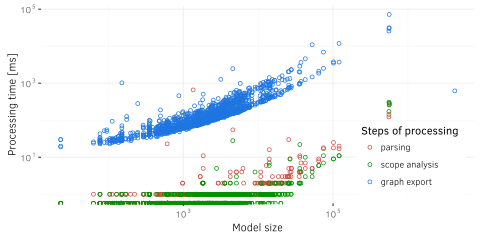
\includegraphics[width=\textwidth]{import-steps.pdf}
  \caption{The characteristics of the import steps.}
  \label{fig:import-steps}
\end{figure}

\Cref{fig:import-steps} shows the characteristics of these three steps. Since even the longest source codes can be written in one line, instead of the source lines of code I have chosen the number of nodes in the transformed subgraph as the horizontal axis. The vertical axis represents the time (in milliseconds) required to perform the given transformation step. Note that both axes are logarithmic.

In order to present an accurate and wide-range measurement, I have selected the repository of the Tresorit web client~\cite{tresorit-webclient}. The current version of this repository contains 780 JavaScript files, with 75\,907 lines of actual code in total. This results in 8\,437\,838 graph nodes.

Since the source code contains language elements not yet standardized, I transpiled the files before they are parsed by the Shift parser. This step is not calculated in the benchmark. The resulting files are then imported into the database one-by-one, sequentially, thus the parallel optimizations are not present in this measurement.

Based on~\Cref{fig:import-steps} the time requirement of the parsing and scope analysis steps are negligible compared to the third step. Iterating and storing the elements of the ASG in the graph database shows polinomial correlation with the size of the graph. It is also visible that most of the files are parsed under one second, which makes this approach useable in real-life usage.

These results are based on two separate, sequential, full import of the source code repository.

\subsection{Connecting the Subgraphs}
% TODO write or hide

\subsection{Dead Code Search}
% TODO write

\begin{figure}[!htb]
  \centering
  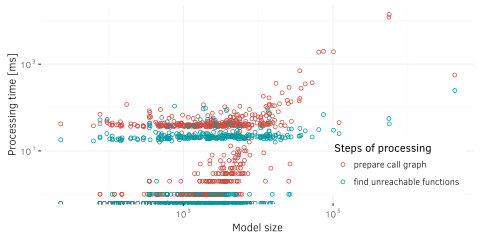
\includegraphics[width=\textwidth]{deadcode-search.pdf}
  \caption{The characteristics of dead code search.}
  \label{fig:deadcode-search}
\end{figure}

\subsection{ASG to CFG Transformation}
In order to measure the characteristics of the CFG transformation, I have imported the source files of the Tresorit web client one-by-one and executed the CFG transformation queries for that one file.

\begin{figure}[!htb]
  \centering
  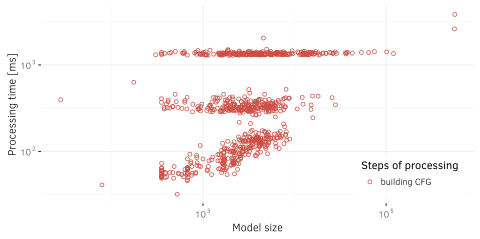
\includegraphics[width=\textwidth]{build-cfg.pdf}
  \caption{The characteristics of building the CFG.}
  \label{fig:build-cfg}
\end{figure}

\Cref{fig:build-cfg} shows that the measurements are clustered into three parts. There are at least two explanations for this:

\begin{itemize}[topsep=0pt]
  \item The number of CFG transformations implemented in the prototype framework is low. Since there are measurements in every cluster for a great amount of model sizes, it is possible that the composition of the files are different in each cluster.

  This would mean that the top cluster --- implementing business logic --- contains more nodes to transform, while the files in the bottom cluster --- mostly describing interfaces and proxies --- contain less.

  \item The transformation is executed in a parallel manner. If two transformations cause a deadlock in the database, they are canceled and tried again later. It is also possible that subgraphs containing more transformable nodes by the framework are processed slower. The slower the transformations are, the more deadlocks may happen, resulting in slower overall performance.
\end{itemize}

It is also unexpected to have the top two clusters show no correlation with the size of the resulting graph size. This phenomenon can be explained with the reasons above or with the way Neo4j executes the declarative transformations.

Since the CFG transformation in the framework is far from finished, deeper examination of the results is subject to future work.


\section{Threats to Validity}
\label{sect:evaluation-threats}
Although I carefully designed and executed each measurement, there might have been factors beyond control that influence the results yielded. In this section, I try to list the possible mistakes and also discuss the steps taken to mitigate their effects.

\subsection{Benchmarking in the Cloud} As a multiple access system, the virtual servers in the cloud can be easily affected by neighboring virtual machines using the same resources. The virtual machine manager can also limit the usage of these resources, if the machines disturb other ones. One can neither control the resources assigned to the machines, nor influence their precise geolocation and connections.

My mitigation strategy is to run the benchmarks multiple times and treat their median as the correct value.

\subsection{Methodological Mistakes} It is possible that I made mistakes while implementing the approach. It may not adhere to the specification correctly, perform the transformations correctly or measure correctly.

To check the validity of the results, I checked the results manually and with others tools.

\subsection{Measurement Mistakes} I may have committed mistakes in the measurements or was led to the wrong conclusions evaluating these mistakes.

\chapter{Future Vision}
\label{chap:future-vision}

\chapter{Conclusions}
\label{chap:conclusions}

My main objective was and still is to provide a soulution for reducing the time required for a global, codebase-level reevaluation of static analysis after a change occurs.

The created framework can transform a rather large source code repository as a whole into a graph representation and maintain it subsequently. It is fount that the approach is suitable for performing code convention compliance checks and for executing static analysis tests on the graph representation.

This approach is also utilizes incremental processing with file-level granularity, speeding up the static analysis. Based on my measurements the framework is fast enough to help its users with fast changing code repositories.

Once the framework contains enough transformations and queries for handling the language, it can extend the everyday toolkit of developers.

\section{Summary of Contributions}
I presented an extensible proof of my novel concept to perform incremental static analysis on dynamic source code repositories based on graph transformations. My proposal is based on software code modeling, model transformation and graph pattern matching. The feasibility of the approach was evaluated using manual validation and benchmarking.

\subsection{Scientific Contributions}
I have achieved the following scientific contributions:

\begin{itemize}[topsep=0pt]
	\item Proposed a novel architecture for building an incremental static analyzer using freely available components.
	\item Proposed an approach to transform JavaScript source code repository into a connected graph model.
	\item Provided an algorithm to update the graph data model incrementally.
\end{itemize}

\subsection{Practical Accomplishments}
I have also achieved the following practical accomplishments:

\begin{itemize}[topsep=0pt]
	\item Created an extensible incremental static analysis framework.
	\item Developed a tool for transforming JavaScript source code into graph data model.
	\item Designed a benchmark evaluating the approach.
\end{itemize}


\backmatter{}
\pagenumbering{roman}
\setcounter{page}{\thesavepage}

\chapter*{Acknowledgments}
\addcontentsline{toc}{chapter}{Acknowledgments}
\label{chap:acknowledgments}
\thispagestyle{plain}

First, I would like to thank Dr. István Ráth and Zoltán Ujhelyi for providing the scientific foundations for my research and insight into software model verification.

I would like to thank my supervisors Ádám Lippai, Dávid Honfi, and Gábor Szárnyas for their friendly advice and enthusiasm. Also, I wish to express my gratitude to all my colleagues at Tresorit and the Fault Tolerant Systems Research Group who provided numerous valuable observations and suggestions. Especially Soma Lucz and Tamás Hegedűs for their input, energy and time.

Last but not least, I am deeply grateful to my family and friends for their continuous support.


%\section*{Awards}
%I am also thankful for the two awards supporting my work.
\vfill

\paragraph{MTA-BME Lend\"ulet}
This work was partially supported by the MTA-BME Lend\"ulet Research Group on Cyber-Physical Systems.

\paragraph{Microsoft Azure for Research Award}
This report was supported by Microsoft Azure making it possible to use cloud resources with ease.

\paragraph{New National Excellence Program}
This report was supported by the ÚNKP-16-2-I. New National Excellence Program of the Ministry of Human Capacities.

\begin{center}
\includegraphics[width=0.3\textwidth]{include/figures/min_en.jpg}
\end{center}


\listoffigures*\addcontentsline{toc}{chapter}{List of Figures}
\listoftables*\addcontentsline{toc}{chapter}{List of Tables}

\printbibliography{}

\appendix
\chapter*{Appendix}\addcontentsline{toc}{chapter}{Appendix}


\label{page:last}

\end{document}
